\documentclass[letterpaper, 10 pt, conference]{ieeeconf} 
\IEEEoverridecommandlockouts 
\overrideIEEEmargins                                      % Needed to meet printer requirements.
\usepackage{booktabs}
\usepackage{subfigure}
\usepackage{natbib}
\usepackage{graphicx}
\usepackage[ruled]{algorithm2e}
\title{\LARGE \bf
Interpreting Multimodal Referring Expressions in Real Time}
\author{Miles Eldon$^{1}$ and Stefanie Tellex$^{1}$
\thanks{$^{1}$Computer Science Department, Brown University}
}

\usepackage{amsfonts, amssymb, amsmath}
\usepackage[usenames,dvipsnames]{color}
\newcommand{\stnote}[1]{\textcolor{Blue}{\textbf{ST: #1}}}
\newcommand{\menote}[1]{\textcolor{Red}{\textbf{ME: #1}}}

\begin{document}

\maketitle
\thispagestyle{empty}
\pagestyle{empty}

\begin{abstract}
Robots that collaborate with humans must be able to identify objects
used for shared tasks, for example tools such as a knife for
assistance at cooking, or parts such as a screw on a factory floor.
Existing work has addressed this problem in single modalities, such as
natural language or gesture, but a gap remains in creating real-time
multimodal systems that simultaneously fuse information from language
and gesture in a principled mathematical framework.  We define a
multimodal Bayes' filter for interpreting referring expressions to
objects using language and gesture in real time.  Our approach outputs
an estimate of which object the person was referencing several times
per second, enabling a robot to dynamically respond with backchannel
feedback while a person is still communicating.  We collected a new
RGB-D and audio dataset of people referring to objects in a tabletop
setting and demonstrate that our approach successfully integrates
information from language and gesture in real time to quickly and
accurately identify objects continuously.  
\end{abstract}

\section{INTRODUCTION}

In order for humans and robots to collaborate in complex tasks, robots
must be able to understand people's references to objects in the
external world.  For example, a robotic cooking assistant might fetch
ingredients and tools, while a robotic factory assistant could deliver
a part or a hospital robot could deliver water to a bedridden patient;
Figure~\ref{fig:example} shows a robot handing a tool to a worker in a
factory.  To refer to objects, people use a combination of language,
gesture, and body language such as eye gaze and looking.  People
provide these signals continuously, and a person's reference can
quickly change based on new information about the domain.  Moreover, a
human listener responds to these signals as they are given using {\em
  backchannels}, for example nodding their head when they understand
and looking confused or interrupting to ask a question when they do
not.  \citet{clark96} refers to this continuous dance as {\em joint
  activity} and compares language use to playing a duet because of its
collaborative nature, where both parties act to establish common
ground and reduce uncertainty.  Language and gesture co-occur and the
relative timing of speech and gesture is critical for accurate
understanding.

In contrast, many existing unimodal models that do not integrate
information from language and gesture~\citep{matuszek14, tellex11,
  kollar10} , even though people fluidly use language and gesture
together.  Approaches that fuse information from language and
gesture~\citep{matuszek14} do not take into account that information
appears to the system over a period of time.  These approaches make it
impossible for a robot to provide back-channel feedback, because of
the length of time required to interpret the communication and because
of the inability to interpret partial utterances.

\begin{figure}
\centering
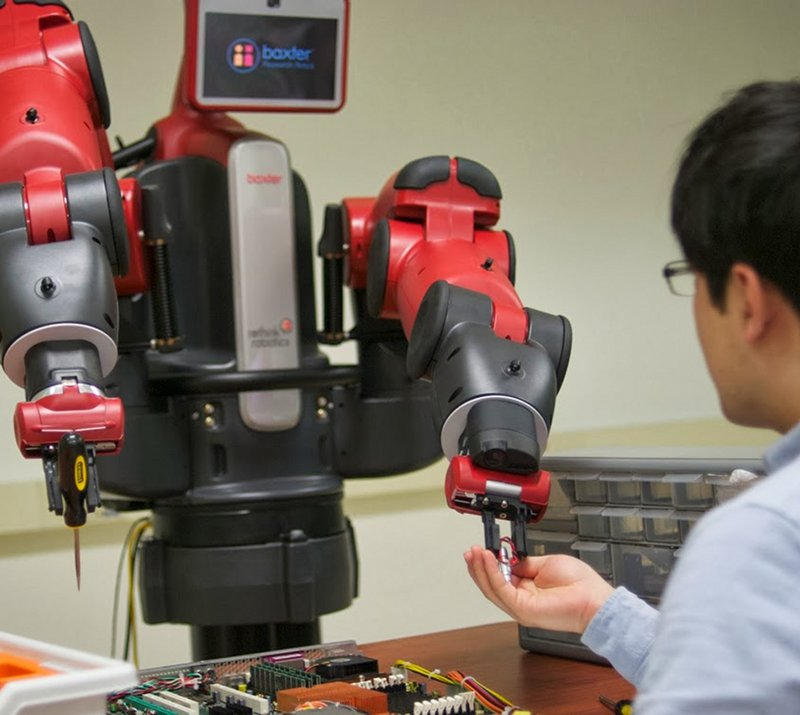
\includegraphics[width=1\linewidth]{figures/baxter_scene_cropped.jpg}
\caption{Robots that collaborate with people need to understand their
  references to objects in the environment.  For example, if a person
  asks for a tool using language and gesture, the robot needs to
  interpret the person's reference in order to pick up the correct
  tool.\label{fig:example}}
\end{figure}


Taking into account time is important because it is the foundation of
seeing language and conversation as a joint activity embedded in time.
Responding quickly to a person's input makes interaction more fluid
and enables a robot to provide back-channel feedback based on its
ability to understand: when it is confident, it can indicate that it
is confident, and when it is unsure, it can indicate that.  This
backchannel feedback could elicit appropriate responses from the
person: they will move to the next task when the robot understands, or
provide more information to disambiguate when the person is confused.

To provide a foundation for these capabilities, we propose a Bayes'
filtering approach for interpreting multimodal information from
language and gesture~\citep{thrun08}.  Our framework relies on a
factored observation probability that fuses information from language,
hand gestures, and head gestures in real time to continuously estimate
the object a person is referring to in the real world.  We demonstrate
our model in simulation, as well as providing quantitative results on
a real-world RGB-D corpus of people referring to objects in the
environment.  These results demonstrate that our approach quickly and
accurately fuses multimodal information in real time to continuously
estimate the object a person is referencing.  We describe how this
approach can be used to program backchannel responses and demonstrate
these responses on a real robot.


\section{RELATED WORK}

\citet{clark96} proposed that conversation is a {\em joint activity},
a coordinated, collaborative processes akin to playing a duet or
performing a waltz.  The two participants must establish {\em common
  ground}.  Common ground in dialog is distinct from symbol
grounding~\citep{harnad90}, which is the problem of mapping from
language to aspects of the external world.  Common ground refers to
the process of two conversational participants establishing joint
understanding about the beliefs of the others.  To establish common
ground, people use {\em backchannel} feedback, such as head nods,
looks of confusion, as well as explicit request for clarification such
as asking a question.  These mechanisms enable the participants in a
conversation to engage in a feedback loop to iteratively establish
common ground as the conversation progresses.  Our approach for
interpreting language and gesture in real time provides a foundation
for producing backchannel feedback with a robot, pointing toward
increased robustness as a person and robot iteratively establish
common ground and actively communicate to reduce errors.

A large body of work focuses on language understanding for
robots~\citep{macmahon06, dzifcak09, kollar10, matuszek12}.  This work
does not take into account the continuous nature of natural language
input.  \citet{guadarrama14} presents a framework for interpreting
open-domain references to objects but focuses on interpreting language
rather than language combined with gesture.  \citet{cantrell10}
presented a framework for understanding language incrementally in real
time dialog but did not use gesture and did not use a corpus-based
evaluation.  Our approach is related to \citet{holladay14} but focuses
on interpreting a person's gestures rather than enabling a robot to
generate pointing gestures.

Many existing approaches for interpreting gesture rely on fixed
vocabularies of gesture, such as ``stop'' or
``follow''~\citep{waldherr00, marge11} without a principled way for
fusing information from language and gesture.  Our work unifies
language and gesture interpretation into a single mathematical
framework, and focuses on parameterized gestures such as pointing.




\citet{matuszek14} presented a multimodal framework for interpreting
unscripted references to tabletop objects using language and gesture.
Our approach similarly focuses on tabletop objects but uses language,
gesture, and head pose, and integrates these disparate data sources
continuously over time using a Bayes' filtering framework.  This
approach enables the robot to continuously process new information and
produce an estimate that converges over time to the correct object as
new information is observed from the person.  

LP and ICMI stuff

POMDP dialog (Steve Young cites gesture stuff.)

Matthias. 

\citet{dragan13} created a framework enabling a robot to produce
gesture.  Similarly, \citet{tellex14} described an approach for
enabling a robot to generate language by inverting a semantics
framework.  Our long-germ aim is that by combining these types of
generation approaches with real-time understanding, the robot will
produce back-channel feedback that closes the loop of dialog and
enable it to participate in dialog as a joint activity.

\section{TECHNICAL APPROACH}

Our aim is to estimate a distribution over the object that a person is
referring to given language and gesture inputs.  We frame the problem
as a Bayes' filter~\citep{thrun08}, where the hidden state,
$\mathcal{X}$, is the set of $m$ objects in the scene that the person
is currently referencing. The robot observes the person's actions and
speech, $\mathcal{Z}$, and at each time step estimates a distribution
over $\mathcal{X}$:
\begin{align}
  p(x_t | z_0 \dots z_{0:t})
\end{align}


To estimate this distribution, we alternate performing a time update
and a measurement update.  The time update updates the belief that the
user is referring to a specific subset of objects given previous
information:
\begin{align}
p(x_t | z_{0:t-1}) = \int p(x_t|x_{t-1})\times p(x_{t-1} | z_{0:t-1}) \text{d}x_{t-1}
\end{align}

The measurement update combines the previous belief with the newest observation to update each belief state: 
\begin{align}
p(x_t |z_{0:t}) = \frac{p(z_t | x_t) \times p(x_t | z_{0:t-1})}{p(z_t | z_{0:t-1})} \\\propto p(z_t | x_t) \times p(x_t | z_{0:t-1})
\end{align}

Algorithm~\ref{alg:algorithm} shows pseudocode for our approach.


\subsection{Prediction Model}

%\stnote{Miles, can you check if this math is right?}
%Looks good!
We assume that a person is likely to continue referring to the same
object, but at each timestep has a small probability, $c$, of
transitioning to a different object: 

\begin{align}
p(x_t | x_{t-1}) = \left\{  \begin{array}{ll}
1-c &\mbox{if } x_t = x_{t-1}\\
c &\mbox{otherwise}
\end{array}\right.
\end{align}

In our experiments, $c$ has a value of XXX.  This assumption means
that the robot's certainty slowly decays over time, in the absence of
corroborating information.  Our framework integrates past language and
gesture information but also quickly adapts to new, conflicting
information because it assumes the person has changed objects.


\subsection{Observation Model}

We assume access to an observation model of the form:
\begin{align}
p(z_t | x_t)
\end{align}

Observations consist of a tuple consisting of a person's actions,
$\langle l, r, h, s\rangle $ where:
\begin{itemize}
	\item $l$ represents the observed origin ($l_o$) and vector ($l_v$) for the left arm.
	\item $r$ represents the observed origin  ($r_o$) and vector ($r_v$)  for the right arm .
	\item $h$ represents the observed origin  ($h_o$) and vector ($h_v$)  for head.
	\item $s$ represents the observed speech from the user,
          consisting of a list of words. Duo to the nature of current
          methods of speech recognition, we maintain all recognized
          speech from the previous XXX seconds as the current speech
          input.
	\end{itemize}

Formally, we have:
\begin{align}
p(z_t | x_t) &= p(l, r, h, s | x_t)\\
\intertext{We factor assuming that each modality is independent of the others given the state (the true object that the person is referencing):}
p(z_t | x_t) &= p(l | x_t) \times p(r | x_t) \times p(h | x_t) \times p(s | x_t)
\end{align}

\noindent The following sections describe how we model each type of
input from the person.

\noindent{\bf Gesture.}  We model pointing gestures as a vector
through three dimensional space. We calculate the angle between the
gesture vector and the vector from the gesture origin to the mean of
each cluster, and then use the PDF of a Gaussian ($\mathcal{N}$) with
trained variance ($\sigma$) to determine the weight that should be
assigned to that object. We define a function $\mbox{A}(o, p_1, p_2)$ as the
angle between the two points, $p_1$ and $p_2$ with the given origin,
$o$.  Then 
\stnote{I'm confused -- what is the third parameter to the Gaussian?}
\menote{It's the observed data, so its the probability of seeing the third argument with the given mean and variance}
\stnote{So $\Phi$ is introduced here without being defined.  I'm not sure what it means.}
\begin{align}
p(l | x_t) \propto \mathcal{N}(\mu_l=0, \sigma_l,\Phi(l_o, l_v, x_t))\\
p(r | x_t) \propto \mathcal{N}(\mu_r=0, \sigma_r,\Phi(r_o, r_v, x_t))
\end{align}

If the person's arm is more than a certain angle away from the table,
we assume they are referring to none of the objects, and perform an
update.  As a result, these gestures do not effect the robot's
estimate of the objects being referenced.

\noindent{\bf Head Pose.}
Head pose is modeled in the same manner as arm gestures.
\begin{align}
p(h | x_t) \propto \mathcal{N}(\mu_h=0, \sigma_h,\Phi(h_o, h_v, x_t))
%p(h|x_t) = [\displaystyle \prod_{q \in x_t} \mathcal{N}(\mu_h=0, \sigma_h, \Phi(h_o,h_v, q))]^{(\frac{\sum_{x'\in\mathcal{X}} len(x'_q)}{len(x_q)})}
\end{align}


\noindent{\bf Speech.}  We model speech as a bag of words. We
take the words in a given speech input and count how many words in
this text match descriptors (denoted $x_d$) of specific objects.
\begin{align}
p(s |x_t) = \displaystyle \prod_{w \in s} p(w | x_t)
\end{align}


\subsection{Null Words and Gesture}

\stnote{Broaden this to talk about words and gesture}
When no words are spoken, we assume a null word which has a uniform
distribution over the objects.  This effect means that spoken words
cause a discrete bump in probability according to the language model,
which then decays over time.  

\subsection{Training Model Parameters}

\stnote{Miles, can you rewrite this section?  I think model parameters
  are tuned by hand right now, and not learned from data.}

We train model parameters by fitting each factor to an annotated
training corpus.  We collected a dataset of people referring to an
object, including language and gesture.  We instrumented human
annotators with a microphone and initialized the gesture tracker.
Then we instructed them to refer to an object which we indicated with
a laser pointer; using a laser pointed meant that we avoided using
language and gesture ourselves to refer to the object.  We periodically
changed the object to refer to, to simulate a dialog where the person
periodically refers to different objects.  For example, the robot
could be acting as a cooking assistant and retrieving different
ingredients, or in a hospital fetching water, a phone, or a book for a
patient recovering from surgery, who is unable to get out of bed.  We
used this real-world dataset to train and evaluate our model.

\begin{algorithm}
    \DontPrintSemicolon
    \KwIn{$bel(x_{t-1}), z_t$}
    \BlankLine
    \KwOut{$bel(x_t)$}
    \BlankLine
    \For{ $x_t$} {
      $\bar{bel}(x_t) = \displaystyle\prod_{x_{t-1}} p(x_t|x_{t-1})*bel(x_{t-1})$
      \BlankLine
      \textbf{if not} is\_null\_gesture(l)
      \BlankLine
      \Indp$\bar{bel}(x_t) = p(l | x_t) *  \bar{bel}(x_t)$
      \BlankLine
      \Indm\textbf{if not} is\_null\_gesture(r)
      \BlankLine
      \Indp$\bar{bel}(x_t) = p(r | x_t) *  \bar{bel}(x_t)$
      \BlankLine
      \Indm\textbf{if not} is\_null\_gesture(h)
      \BlankLine
      \Indp$\bar{bel}(x_t) = p(h | x_t) *  \bar{bel}(x_t)$
      \BlankLine
      \Indm\For{$w \in s$}{
      	$\bar{bel}(x_t) = p(w | x_t) *  \bar{bel}(x_t)$
      }
      $bel(x_t) = \bar{bel}(x_t)$

    }
    \BlankLine
\caption{Interactive Bayes Filtering Algorithm} 
\label{alg:algorithm}
\end{algorithm}

\begin{figure*}
\centering
\subfigure[Ambiguous gesture.]{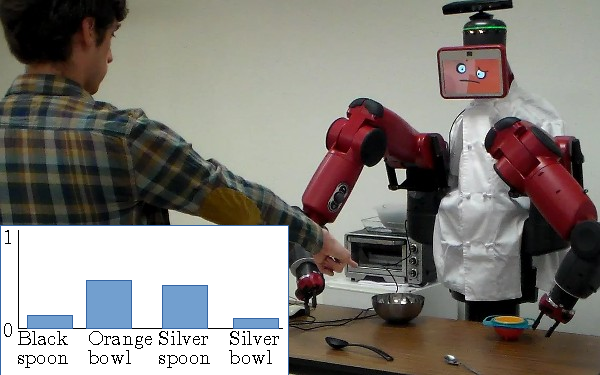
\includegraphics[width=0.4\linewidth]{figures/cartoon1.pdf}}
\subfigure[Clarification with language.]{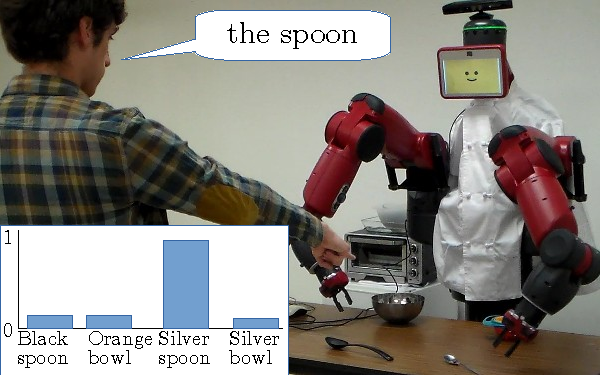
\includegraphics[width=0.4\linewidth]{figures/cartoon2.pdf}}
\caption{After an ambiguous gesture, the model has a uniform
  distribution between two objects (a).  Clarification with language
  causes a probabilistic update leaving the model highly confident it
  has inferred the correct object (b). \label{fig:cartoon}}
\end{figure*}

Figure~\ref{fig:cartoon} shows an example of the system's execution.
The person's gesture is ambiguous, but information from language, that
is itself ambiguous (because there are two bowls in the scene, enables
the system to infer the correct object.  Although in this example we
are demonstrating the approach at two specific timesteps, the system
is updating its distribution continuously, enabling it to fuse
language and gesture as it occurs and quickly updating in response to
new input from the person, verbal or nonverbal.  Our approach runs at
30Hz, continuously outputting an estimate of the object the person is
referencing.  \stnote{Is 30Hz correct?}

\section{EVALUATION}

We evaluate our model in simulation, comparing the full model to
versions without multimodal information.  Additionally we assessed its
performance on an RGB-D audio and video corpus of people referring to
objects.  Finally we created an end-to-end robotic demonstration,
demonstrated in the video attachment to our paper, and available
online\footnote{video reference}. 

\subsection{Simulation Results}

We evaluated our approach in simulation by generating data from the
model and assessing its accuracy at estimating the object being
referenced.  We generate simulated pointing data for each hand, the
face, as well as spoken utterances at each timestep according to the
model parameters.  We then use these parameters to update the system's
estimate of the object being referred to.
Table~\ref{table:sim_results} shows the results.  Our accuracy metric
is the fraction of time that the robot is pointing at the correct
object.  We report performance using language alone, gesture alone,
and language combined with gesture.  These results demonstrate that
the system is successfully able to fuse multi-modal information to
achieve higher accuracy than each modality alone, but do not show
performance in the real world.  While a gesture and language output
probabilistically referencing the true object are produced at each
time step in simulation, the multimodal accuracy is robust to severe
increases in single-modal noise.  \stnote{Can we create results
  demonstrating this?  For example, a few more columns in table I for
  different levels of language and gesture noise?}\menote{Yeah, I can look into it}


\begin{table}
\centering
\caption{Simulation Results\label{table:sim_results}}
\begin{tabular}{lr}
Language alone &  36.5\%\\
Head alone & 50.9\%\\
Arms alone & 62.4\%\\
Language and gesture &  65.7\%
\end{tabular}

\end{table}

\subsection{Real-World Corpus-Based Results}

\begin{figure}
\parbox{1\linewidth}{~\\~\\~\\~\\}
\caption{Scene from our dataset.\label{fig:corpus_scene}}
\end{figure}

Our real-world experiments measured our algorithm's performance when a
person referred to an object visually and with gesture.  The subject stood in front of a table with four objects placed approximately one foot apart, forming four corners of a square,
as shown in Figure~\ref{fig:corpus_scene}.  We instructed subjects to ask for the indicated object in the most naturally way possible, using whatever combination of gesture and language they felt was appropriate. We indicted the object to refer to using a
laser pointer, and we periodically shifted to a different object on a
predetermined schedule.  They wore a microphone to pick up
high-quality audio, and we tracked their body pose using the NITE
tracker~\citep{openni}.  We used a single Kinect that was able to capture both the user and the table.

We used the HTML5 Speech Recognition package in conjunction with Google Chrome to recognize speech.
This package reports incremental output in real time as recognition
proceeds, and we perform a model update each time a new word is
perceived.  Our training procedure works on actual speech recognition
results rather than transcript speech, enabling the algorithm to adapt
to the errors produced by the recognizer: if it returns ``cake''
instead of ``cup,'' our language model will correctly associate the
word ``cake'' with the ``cup'' object.

Results appear in Table~\ref{table:real_results}.  

\stnote{We need to add:
\begin{itemize}
\item what the numbers mean.  (Is this still \% of time that it was correct?)
\item Table for  correctness at the end of the interaction (offset by something, as we talked about
\item Confidence intervales
\item Random.  I think it's 25\%, and if that's right we can just add a row.
\end{itemize} 
}

\menote{A few things of interest we should note: Head results are poor because NITE doesn't perform fine grained head tracking. Arms have a much higher variance based on how much users rely on gestures vs specific language. I don't know how much we get into that, but I've seen 45 - 95\% accuracy on gesture, while I've seen 75-98\% multimodal, which will be shown once I add the confidence interval to the table, but we might want to discuss}
\begin{table}
\caption{Real-world Results\label{table:real_results}}
\centering
\begin{tabular}{lr}
\toprule
Language only &  35\%\\
Gesture only  &  75\%\\
Head only     &  24\%\\
Multimodal (Language and Gesture) & {\bf 85\%}\\
Multimodal (All) &  65\%\\
\bottomrule
\end{tabular}
\end{table}

\subsection{Robotic Demonstration}

Because our approach enables a robot to quickly and constantly monitor
a person's references to an object, a robot can respond to these
estimates in real time.  We demonstrate this behavior by enabling
Baxter to demonstrate its certainty about what object is being
referenced, this eliciting more feedback from the person.  When the
robot is very unsure, its arm moves back and forth between the
candidate objects.  When it is sure, then it moves with more
precision.  The video shows this behavior, as a person provides more
information about what object is being referred to by the person.

\section{CONCLUSION}

We have demonstrated a Bayes' filtering approach to interpreting a
person's multimodal language and gesture references to objects
continuously in real time.  Our approach enables a robot to understand
a person's references to objects in the real world.

In the future we plan to expand our language model to incorporate
models of compositional semantics and lower-level visual features so
that the robot is not limited to prespecified object models.
Additionally we aim to enable the robot to generate back-channel
feedback based on its model.  \citet{dragan13} created a framework for
generating legible gesture, and we anticipate that enabling a robot to
respond by pointing as in \citet{holladay14} when it is sure and
reflecting its confusing when it is unsure.  Closing the loop will
enable the human-robot dyad to increase efficiency and enable the
robot to accurately infer the human's intent, naturally eliciting more
information when it is confused and indicating that it has understood
when it is sure.  This paper represents steps toward continuous
language understanding and the vision presented by \citet{clark96} of
language as joint activity.


\bibliographystyle{abbrvnat}
\bibliography{main}



\end{document}
